\chapter{Molecular modeling of biological membranes}
\label{chap:methods}

Biological membranes are of a great interest in biology and biophysics. 
The tools and methods that enable their research have greatly evolved over the last decades. 
Nowadays, there is a plethora of membrane models and experimental methods, 
each having its benefits and drawbacks \citep{REF} \todoi{1-2 chosen reviews, everything else in prev chapter}
(see section~\ref{sec:modelmemb} in chapter~\ref{chap:intro} for a detailed overview). 

Molecular simulation can be considered as one of the newer approaches in this field. 
Starting with simple membrane models \citep{REF} \todoi{REF: few old/new simulation works},
simulation of membranes has evolved into a field of computational biophysics
that is capable of answering fundamental questions.
The recent progress in computational resources and algorithms
has allowed the simulations to grow in spatial scales and composition complexity
bringing more relevance for applications in biology. \citep{REF: CECAM workshop} \todoi{REF to CECAM workshop 2018 Lugano}

Molecular dynamics simulations of biological membranes employ classical particle-based models of molecules. 
Vast majority of the models are built using classical non-polarizable particles, 
each representing an individual atom (atomistic models), 
or a group of atoms (united-atom or coarse grained models). 
The following classical models belong among the most popular in membrane modeling:
\begin{itemize}
 \item Atomistic
 \begin{itemize}
   \item CHARMM \citep{klauda10}
   \item Slipids \citep{jambeck12, jambeck12b}
   \item OPLS lipids by \citet{maciejewski14}
   \item Lipid14 \citep{dickson14}
  \end{itemize}

 \item Coarse grained
 \begin{itemize}
   \item MARTINI \citep{marrink07}
   \item Berger \citep{Berger97}
   \item CHARMM-UA \citep{lee14}
  \end{itemize}
\end{itemize}

Despite all successes and valuable insights simulations have provided, 
there is still a large room for possible improvements of the current simulation models. 
For example, recent studies by \citet{botan15, catte16} has shown 
that both structure and interaction of phospholipid models require further optimization 
in order to become capable of interpreting solid state NMR experiments. 
In particular, we have discovered that 
the lack of polarizability is a major issue in any of the models 
from the above mentioned works \citep{botan15, catte16}
when interactions with charged moieties become important. 
Several possible ways for embedding polarizability into simulations, both explicit and implicit, 
will be introduced in the following sections. 





\section{Classical molecular dynamics simulations}
\label{section:md}

Classical molecular dynamics simulation provides insight into the dynamics and structure of molecules. 
It is commonly used for generating equilibrium thermodynamic ensembles,
that cas serve as input for statistical methods to extract observable equilibrium quantities. 
Classical MD simulation can be also used to assess the evolution of non-equilibrium states.
Such application is commonly termed as \emph{Steered MD}. 
Molecular modeling, and MD simulation in particular, 
is often combined with experiments,
which helps in their interpretation and provides detailed insight. 

In a MD simulation, the system of interest is propagated numerically in discrete time steps.
Newton equations of motion are used for systems with calssical particles, which form the majority of applications.
Interactions between particles, which often represent individual atoms, 
are described by an approximate interaction potential, also called \emph{force field}. 

The form of the force field varies with the model potentials that are used for the description of the individual interaction components. 
As an example, the interaction potential of AMBER \citep{ferrer13}, a popular model for biomolecules, has the following form:
 % Amber potential energy form:
\begin{eqnarray}  \label{eq:amber}
  V = & \displaystyle \sum _{bonds} K_b (r-r_{0})^2 + \sum _{angles} K_\Theta (\Theta-\Theta_{0})^2 + \\ \nonumber
      & \displaystyle \sum _{dihedrals} \frac{1}{2} V_n (1+\cos(n\phi -\phi_0)) + \sum _{i<j} \left [ s_{ij} ^{VdW} \left( \frac{A_{ij}}{r_{ij} ^{12}} - \frac{B_{ij}}{r_{ij} ^6} \right ) + s_{ij}^q \frac{q_i q_j}{\epsilon \, r_{ij}} \right ]
\end{eqnarray}
The first three terms represent the intra-molecular forces arising from bond stretching, angle bending and dihedral angle torsion. 
The symbols $K$ and $V$ are the force constants that describe the strength of such an interaction,
$r$, $\Theta$ and $\phi$ are the respective dimensions,
and $n$ is the multiplicity of the torsion potential. 

The last terms in the square brackets represent the inter-molecular interactions; the dispersion, or Van der Waals forces, and electrostatic interaction. 
Depending on the model force field, the non-bonded interactions are evaluated only for atoms separated by more than three or four bonds, 
which is here formally introduced through the matrix $s_{ij}$ that modifies the interaction accordingly.

The constants in matrices $A_{ij}$ and $B_{ij}$ represent the strengths of the repulsion and attraction forces 
arising from disperion and the overlap of the electronic clouds of the individual particles.  
The electrostatic interaction is described by the interacting partial charges $q_i$ and by the formally applied dielectric constant $\epsilon$ of the medium, 
which is assumed to be 1 in most force fields for biomolecules. 
In a later section~\ref{section:ecc}, we will show how to modify this interaction 
by changing the dielectric constant $\epsilon$ to include the effects of electronic polarization. 

Note that the interactions are simplified not only by the empirical formulae for the individual contributions, 
but to a large extent also by assuming that the interaction potentials are \emph{pair-wise additive}. 
Especially in the case of the inter-molecular forces, this is a severe assumption, 
which neglects the contributions from three and higher-body interactions. 
It was, however, shown that even such an approximate interaction potential is sufficiently accurate in many cases 
(see the list in the beginning of this chapter for such examples). 

The electrostatic interaction yields the strongest inter-molecular forces. 
In classical MD simulation, the electrostatic interaction is approximated by point charges in the centres of the particles. 
It has non-negligable contributions even from long distances. 
In periodic systems, i.e. in simulations with periodic boundary conditions, 
evaluating contributions from all periodic images is necessary. 
In neutral systems, this is efficiently done by 
summing the long range contributions in Fourier space rather than in real space
using fast algorithms developed for this purpose. \citep{darden93, essman95}

The dispersion interaction in the example empirical interaction potential in Equation~\ref{eq:amber} adopts the form of Lennard-Jones potential, 
which can be also expressed in terms of interaction energy $\epsilon_{ij}$ and the distance of the potential minimum, $\sigma_{ij}$, as
\begin{equation}
   U_{LJ} =  \frac{A_{ij}}{r_{ij}^{12}} - \frac{B_{ij}}{r_{ij}^6} = \epsilon _{ij} \left [ \left (\frac{\sigma _{ij}}{r_{ij}} \right )^{12} - 2 \left ( \frac{\sigma _{ij}}{r_{ij}} \right )^6 \right ] .
\end{equation}
The parameter $\sigma$ separates the regions, 
where the interaction is repulsive (distances smaller than $\sigma$), 
and where they are attractive (distances larger than $\sigma$). 
Such a parameter hence also tells on the size of the spherical particle, 
which has an impact on the balance between electrostatic and Van der Waals forces.

The parameters $\sigma_{ij}$ and $\epsilon_{ij}$ are usually derived for a small set of pairs,
and the parameters for any other pair of particles are derived by using combination formulae. 
The most common combination rules are Lorentz-Berthelot's:
\begin{equation}
 \sigma _{ij} = \frac{1}{2} (\sigma _{ii} + \sigma _{jj}) \, ; \quad \epsilon _{ij} = \sqrt{\epsilon _{ii} \, \epsilon _{jj}} 
\end{equation}









\section{Including polarizability}

\todo{This section can be included-or-omitted at leisure.}
The lack of electronic polarizability in standard MD simulation
force fields has been considered a serious issue since the early days of
lipid bilayer simulations \dots
  Lit. research (history) on how people include polarizability in classical simulations. 

\subsection{Explicit treatment of electronic polarizability}

\todo{This section can be included-or-omitted at leisure.}
 Joint subsection on Drude particles and polarizable dipoles, the most common ways of introducing polarizability explicitly into the MD simulation. 
\ldots rather demanding explicit inclusion
of electronic polarization effects \cite{lucas12,chowdhary13} \dots





\subsection{Electronic continuum correction as implicit treatment of electronic polarizability}
\label{section:ecc}

The theory for accounting for electronic polarization in empirical force fields
was originally developed by \citet{leontyev09} under the name Molecular Dynamics in Electronic Continuum, MDEC. 
The term Electronic continuum correction, ECC, originates in the works by \citet{Pluharova2014, kohagen14, kohagen16, martinek17},
where the rigorously developed theory from \citep{leontyev14} was applied on ionic solutions.
Through the comparison of neutron scattering and/or \emph{ab-initio} data with classical MD simulations, 
the authors developed an array of models for cations an anions, here termed ECC-ions,
that embedded ECC as an implicit model polarizability for electrons. 

\todo{Extensions of this section are relatively easy and possible by incorporating more equations and MDEC theory.}

Electronic continuum correction (ECC) is an implicit model of electronic polarization. 
in which a system of polarizable particles is represented
with an equivalent system of particles with fixed charges
including the effects of electronic polarization \emph{implicitly} in a mean-field way. \citep{leontyev09, leontyev10, leontyev11, leontyev14}
This can be done by a relatively simple transform of the partial charges,
which does not change the form of the formula of the empirical force field (examples in section~\ref{section:md})
making a wrong impression of a \emph{non-polarizable} model again. 
Technically, ECC is similar to the phenomenological scaling of partial charges, 
which was applied in earlier studies of aqueous solutions or ionic liquids \citep{jonsson86,egberts94,beichel14},
in which also other possible effects (e.g. charge transfer) were considered.
In contrast, ECC is a physically well justified and rigorously derived model~\citep{leontyev09, leontyev10, leontyev11, leontyev14}.
The relation for the charges employing ECC model can be formally written as
\begin{equation}  \label{eq:scaling}
 Q^{ECC} = f_q \cdot Q ,
\end{equation} 
where $Q$ and $Q^{ECC}$ are the original and the scaled, \emph{implicitly polarized}, partial charges respectively. 
The relation between the original and the new set of charges 
is, hence, a mere linear scaling with a certain factor, $f_q$, 
which is related to the high-frequency dielectric constant, $\epsilon _{el}$, of the electrons according to
\begin{equation}   \label{eq:scaling_factor}
 f_q = \sqrt{ \epsilon _{el} }
\end{equation} 

The presented Relation~\ref{eq:scaling} is rather a practical way of implementing the ECC polarizability model into the simulation. 
It is equivalent to embedding all atoms into a dielectric continuum 
with the high-frequency dielectric constant of the electrons, $\epsilon _{el}$, providing the same effect.
It is important to note that the value of the high frequency dielectric constant  
is around 2 for almost any biologically relevant environment \citep{leontyev11}. 
This means that even interfaces like biological membranes do not contain discontinuities of the electronic continuum. 
The dielectric discontinuity in a lipid bilayer thus arises only 
from the orientational polarization of the molecules, which is accounted for explicitly in standard MD simulations.  
Therefore, the same correction for the electronic polarizability can be  
applied throughout the lipid bilayer/aqueous solution interface. 
Given that the  high frequency dielectric constant of water is 1.78 (i.e., the square of the refraction index), 
the scaling factor for ions in water is $\approx 0.75$. 





 

 
 



\section{Implicitly polarizable classical MD models of lipids using ECC}
\label{section:ecc-lipids}

Simulations with explicitly polarizable models are generally considered to be computationally too demanding for a practical use in biophysics. 
The models employing ECC, however, are on the same level with classical non-polarizable models with fixed charges, yet they implicitly incorporate electronic polarization. 
The ECC theory was introduced in the above section~\ref{section:ecc}.
In this section, I will demostrate the application of the ECC theory on phospholipids, 
where the effects of polarization yield crucial consequences in the accuracy of the interaction with ions. 

We chose phosphatidylcholine (PC), phosphatidylethanolamine (PE) and phosphatidylserine (PS)
as representants of the most common neutral and negatively charged lipids in plasma membrane \citep{the_review_with_pie_charts_on_my_desk, marsh13}. 
The Lipid14~\citep{dickson14} model was used for POPE and POPC,
and the Lipid17~\citep{lipid17} model, already available from AmberTools \citep{ferrer13},
were used as the starting point for embedding ECC.
It was shown by \citet{botan15, catte16} that such a family of lipid models provides one of the most 
realistic descriptions of the head group order parameters of POPC and their response to ions 
when compared to other available lipid models. 

In the case of POPS, which bears a total negative charge of -1, 
embedding ECC through the linear transform of the partial charges is straightforward. 
The resulting ECC-lipid model of POPS, also denoted as ECC-POPS, 
adopts a formal total charge $-0.75$ in line with ECC and the electronic dielectric constant of water \citep{leontyev14}. 
Note that the formal charge is equal in size to the charges of monovalent ions developed with ECC \citep{Pluharova2014, kohagen14, kohagen16, martinek17}.

While the scaling factor of $f_q = 0.75$ is undoubtedly justified for molecules with a non-zero total charge like ions or POPS,
it is not \emph{a priori} clear what factor shall be used for neutral molecules, i.e. for POPE and POPC in our case.

The partial charges of particles forming molecules in simulations are not physical observables unlike the total charge. 
There is a variety of schemes for assigning partial charges to particles in molecules~\citep{Hu2007}. 
The restrained electrostatic potential method (RESP) is, however, the most common method used in biomolecules~\citep{RESP_paper, Singh1984, dickson14}. 
In practice, it is common that water molecules are included in the RESP calculations, 
and charges are subsequently refined to improve certain experimental observables. 
Although such tweaks do not affect the zero total charge for neutral molecules,
it naturally follows that the effects of electronic polarizability 
may to some extent be present even in standard force fields~\citep{RESP_paper, Singh1984, jorgensen96, ipolq2013, benavides17}. 
We thus conclude that the scaling factor, $f_q$, for partial charges in existing models of neutral molecules does not necessarily follow the relation \ref{eq:scaling_factor}.
It is expected instead, that the scaling factor may adopt a slightly higher value than 0.75. 

The ECC correction was applied on top of the Lipid14/Lipid17 models of POPC, POPE and POPS
by scaling the partial charges of all atoms except acyl tails, 
i.e. the polar parts in phospholipids, head group, glycerol backbone, and carbonyl regions. 
Such a choice was guided by the observed strength of interaction with cations. 
In contrast, the acyl chains do not come in direct contact with ions from the solution, 
and they are already highly optimized to provide a good description of the
hydrophobic part of lipid bilayers \cite{dickson14,ollila16}.
Compared to the acyl tails, the glycerol backbone and the head group regions of phospholipids 
require improvements in any available lipid model~\cite{botan15}.

We found that the optimal value for the scaling factor of partial charges of the neutral molecules from the Lipid14 force field \citep{dickson14}
is $f_q = 0.8$, which is indeed close to 0.75, 
the scaling factor for the ions in water. 
This value was found by comparing the results from the simulations with POPC to the experimental 
NMR data~\cite{akutsu81,altenbach84,scherer89} on the head group order parameter response to the bound charge.
Note that common empirical scaling factors for solutions of monovalent ions in water 
are 0.8 or even higher \citep{benavides17,skinner14,nacleps}.  
In contrast, modern force fields for ionic liquids often employ values around 0.6--0.65, 
which are on the other hand much lower than $\epsilon^{-1/2}_{el}$ \citep{holm14}.

Although scaling of the partial charges improved 
the head group order parameter response and ion binding affinity,
it at the same time has deteriorated certain membrane properties; 
namely the area per lipid generally decreased, often below the experimental values. 
The decrease of the area per lipid is observed to likely arise from a reduced hydration of the lipid head group region
as the polarity of the head group has overall decreased after scaling charges. 

We compensated this effect
by reducing the effective radii of atoms with the scaled charges.
This was explicitly done for POPC by changing the parameters $\sigma$ in the Lennard-Jones potential 
in a similar way as was done previously for the ECC-ions in solution \cite{kohagen14,kohagen16,Pluharova2014}.
Reducing the $\sigma$ parameters of the affected atoms by a factor of $f_\sigma = 0.89$
restored the area per molecule to the level very close to the experiment (Table~\ref{tab:apls}). 
Such optimized parameters $\sigma$ were then used for all ECC-lipids, i.e. also for ECC-POPE and ECC-POPS. 
In addition, the X-ray scattering form factors of POPC, POPE and POPS from simulations remained at a good agreement or even improved with the modifications 
(see Figs.~\ref{simVSexpNOions}, \ref{simVSexpNOions_POPS} and \ref{simVSexpNOions_POPE}). 








\subsection{Structural parameters of model membranes with ECC-lipids: Agreement with experiments} 
 
%%%%%%%%%%%%%%%%%%%%%%%%%%%%%%%%%%%%%%%%%%%%%%%%%%%%%%%%%%%%%%
% problemgsolved: NO line breaks in the caption!
\begin{figure}[tb!] 
  \centering 
  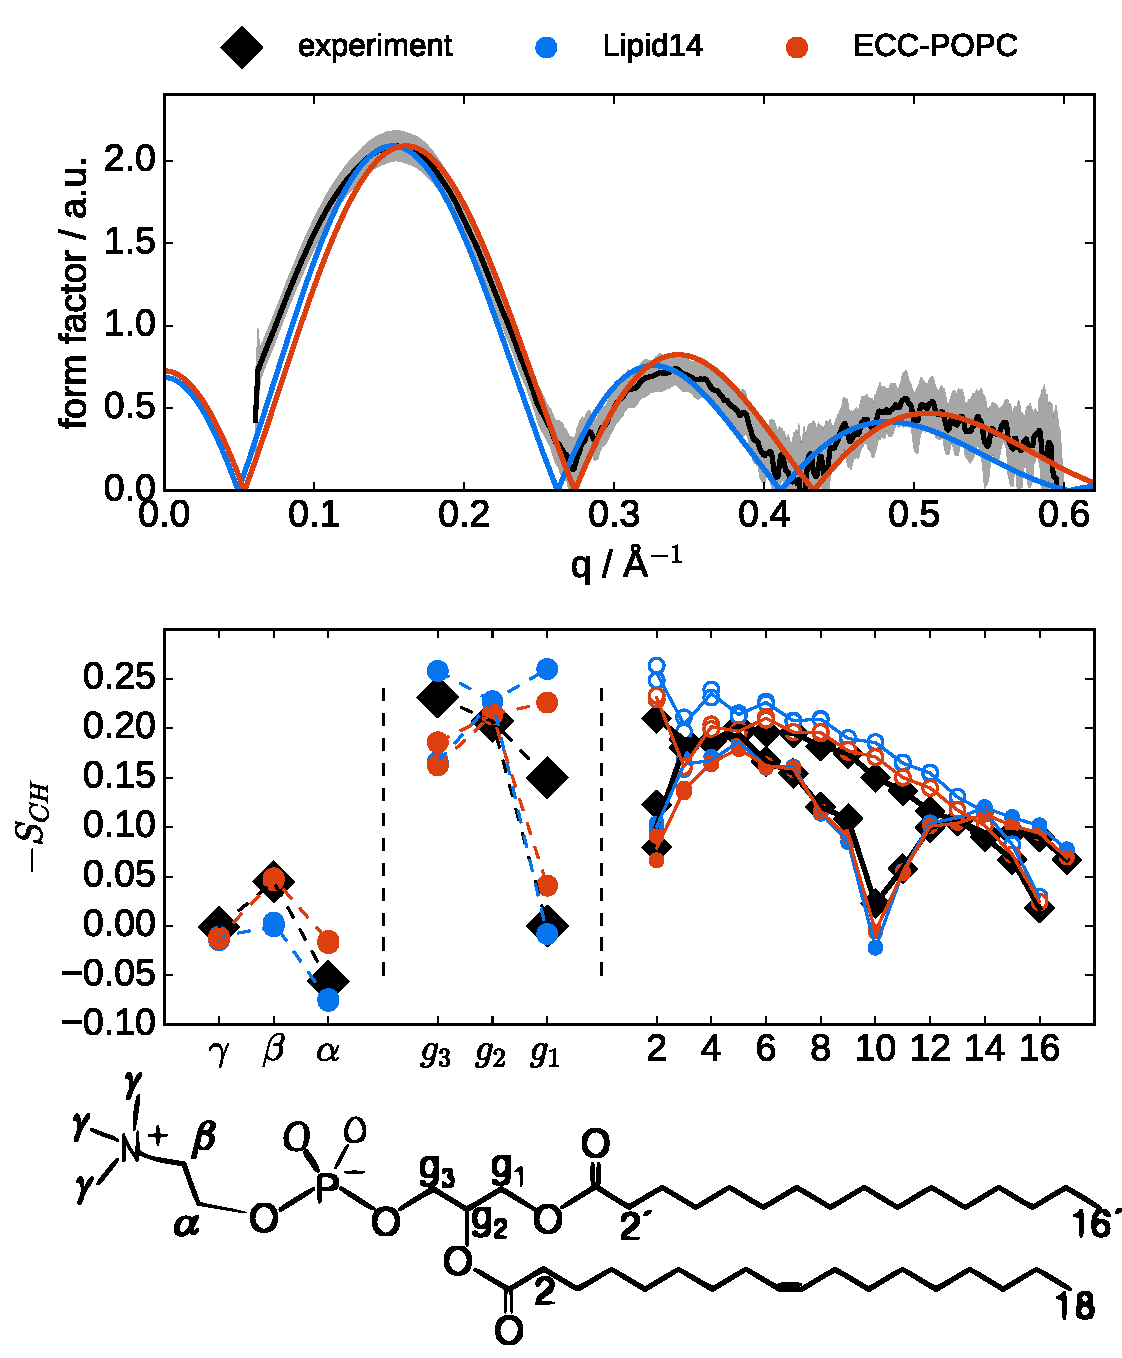
\includegraphics[width=8.2cm]{../img/ecc_popc/Order-parameters_form-factors_exp-L14-ECCL17_q80_sig89_POPC-struct.pdf} 
  \caption{ \label{simVSexpNOions} 
    Top: X-ray scattering form factors from simulations with the Lipid14 \citep{dickson14} and 
    the ECC-POPC \citep{melcr18} models compared with experiments~\citep{kucerka11} at 303~K. 
    Middle: Order parameters of POPC head group, glycerol backbone and acyl chains  
    from simulations with the Lipid14 and the ECC-POPC models 
    compared with experiments \citep{ferreira13} at 300~K. 
    The size of the markers for the head group order parameters correspond to 
    the error estimate $\pm 0.02$ for experiments \citep{botan15,ollila16}, 
    while the error estimate for simulations is $\pm 0.005$
    (Bayesian estimate of 95\% confidence interval \citep{scipy}).
    The size of the points for acyl chains are decreased by a factor of 3 to improve the clarity of the plot.
    Open/closed symbols are used for palmitoyl/oleoyl chains of POPC. 
    Bottom: The chemical structure of POPC and the labeling of the carbon segments. 
  }  
\end{figure} 


\begin{figure}[tb!] 
  \centering 
  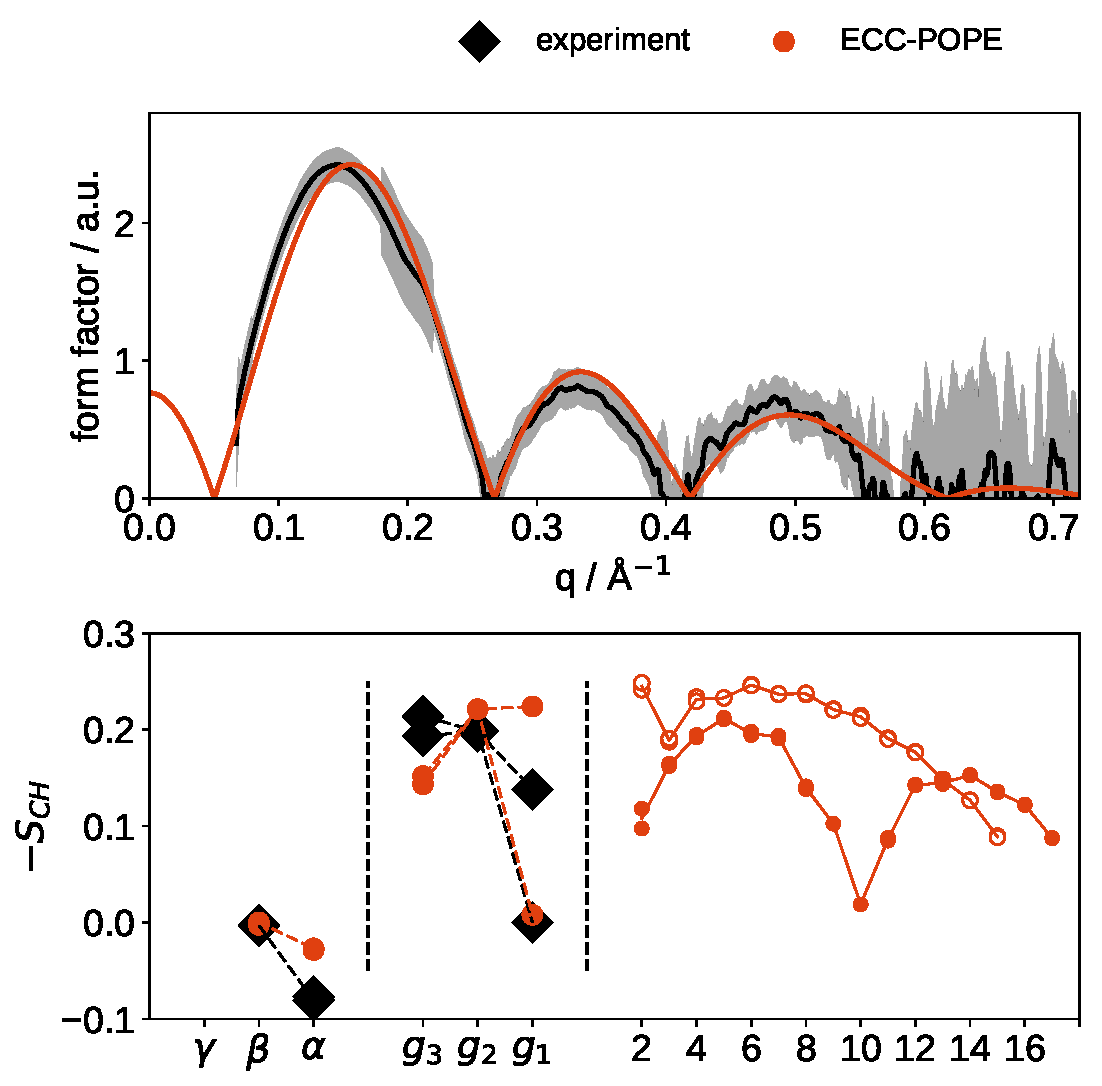
\includegraphics[width=\figwidth]{../img/ecc_pope/Order-parameters_form-factors_exp-ECC-POPE.pdf}
  \caption{\label{simVSexpNOions_POPE} 
    X-ray scattering form factors from simulations with 
    the ECC-lipids model of POPE compared with experiments~\cite{kucerka11} at 313~K. 
    Order parameters of POPE head group, glycerol backbone and acyl chains  
    from simulations with the ECC-lipids model of POPE
    compared with experiments by \citet{gally81} (order parameters of glycerol backbone, labeled \emph{E. coli} membrane at~310\,K, ) 
    and by \citet{seelig76, seelig80} (order parameters $\alpha$ and $\beta$ from DPPE at~341\,K).
    Open/closed symbols are used for palmitoyl/oleoyl chains of POPE. 
  }  
\end{figure} 


\begin{figure}[tb!] 
  \centering 
  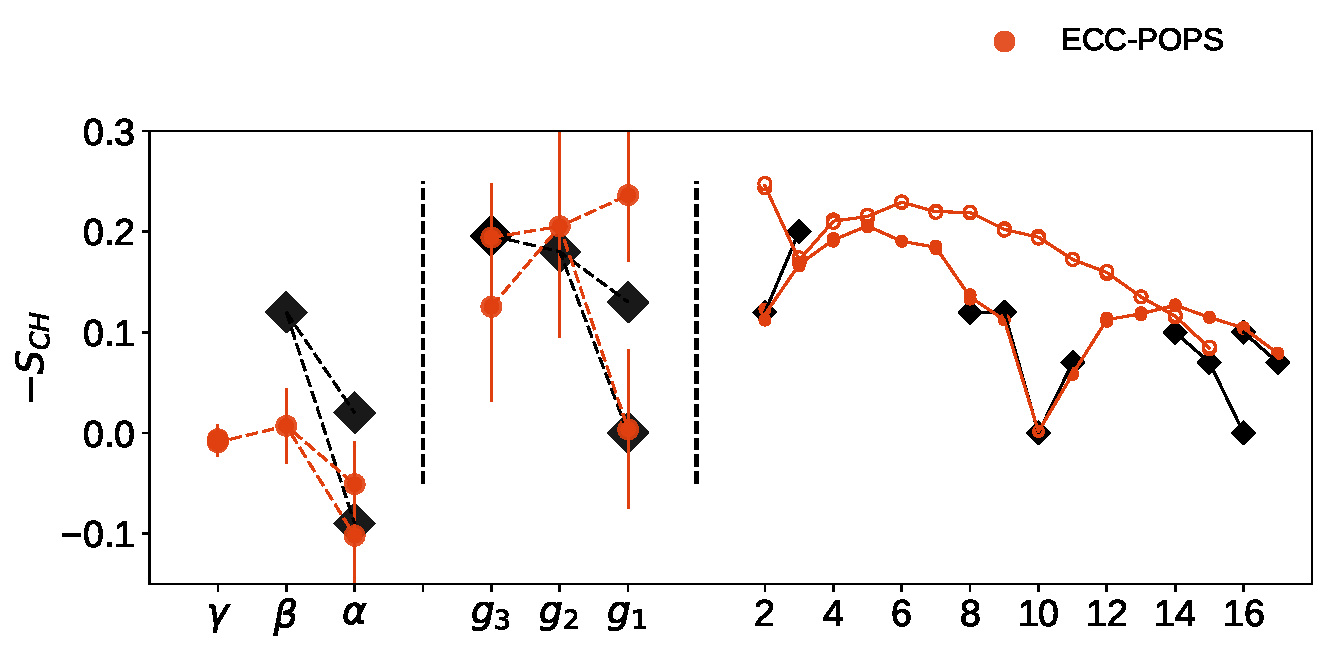
\includegraphics[width=\figwidth]{../img/ecc_pops/order_parameters_actual_pure-POPS.pdf} 
  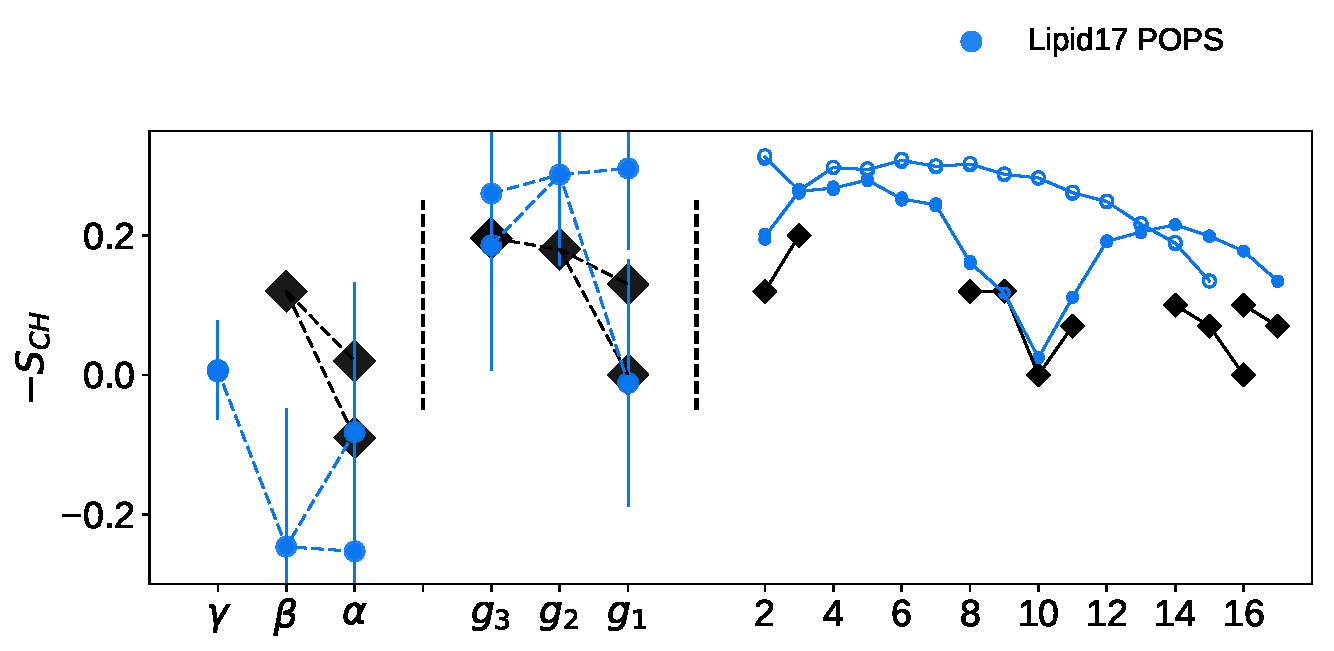
\includegraphics[width=\figwidth]{../img/ecc_pops/l17/order_parameters_actual_pure-POPS.pdf} 
  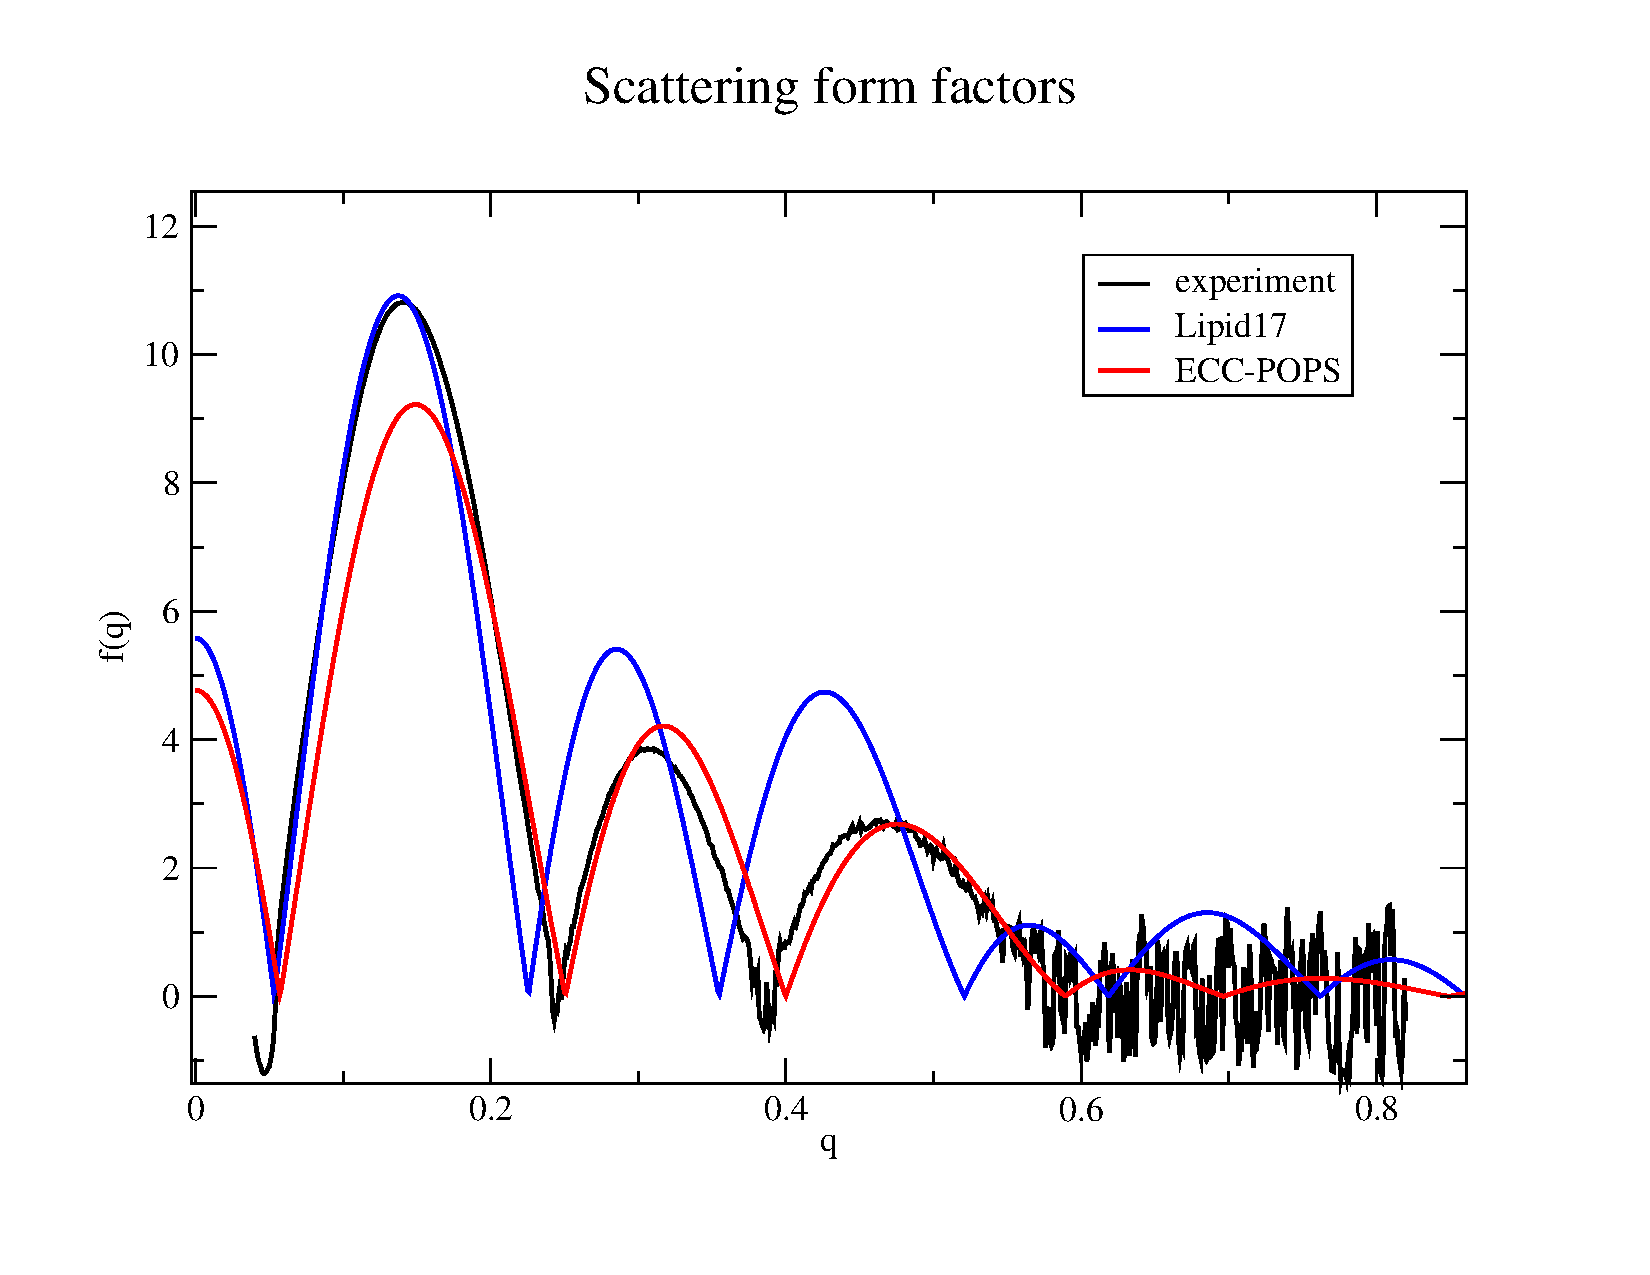
\includegraphics[width=\figwidth]{../img/ecc_pops/form-f_l17-ecc-pops-exp_compar.pdf} 
  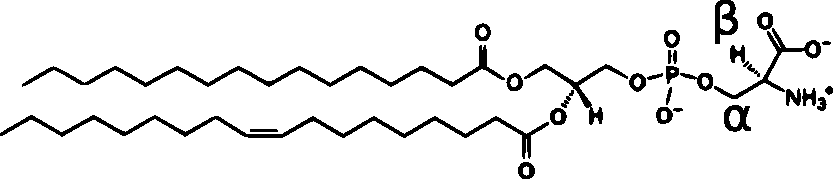
\includegraphics[width=\figwidth]{../img/ecc_pops/pops_chemfig.pdf} 
  \caption{\label{simVSexpNOions_POPS} 
    X-ray scattering form factors from simulations with the Lipid17 \cite{lipid17-future} and 
    the ECC-POPS \citep{melcr18} models compared with experiments~\cite{SDP-CHARMM36_comparison_paper_Samuli-knows} at 298~K. 
    Order parameters of POPS head group, glycerol backbone and acyl chains  
    from simulations with the Lipid17 \cite{lipid17-future} and the ECC-POPS models 
    compared with \emph{experiments at 300~K (check and change)} measured by Tiago Ferriera. 
    Open/closed symbols are used for palmitoyl/oleoyl chains of POPS. 
    The chemical structure of POPS and the labeling of the carbon segments. 
  }  
\end{figure} 
%%%%%%%%%%%%%%%%%%%%%%%%%%%%%%%%%%%%%%%%%%%%%%%%%%%%%%%%%%%%%%
 
\begin{table}[tb!] 
  \caption{Values of the area per lipid (APL) of POPC, POPE and POPS bilayers without additional ions. \label{tab:apls} 
  } 
  \begin{tabular}{l|c c} 
    \multicolumn{3}{c}{POPC} \\
    \hline 
    model          & APL (Å$^2$)   & Temperature (K) \\ 
    \hline 
    Lipid14 POPC                    & 65.1$\pm$ 0.6  &  300 \\ 
    Lipid14 POPC \citep{dickson14}  & 65.6$\pm$ 0.5  &  303 \\ 
    \hline 
    ECC-POPC     \citep{melcr18}    & 63.2$\pm$ 0.6  &  300       \\ 
    \hline 
    experiment (SDP model) \citep{kucerka11} & 64.3  &  303    \\ 
    \hline 
    \\
    \multicolumn{3}{c}{POPE} \\
    \hline 
    model          & APL (Å$^2$)   & Temperature (K) \\ 
    \hline 
    ECC-POPE                 & 56.7$\pm$ 0.8  &  298 \\ 
    \hline 
    experiment   \citep{parsegian89} & 56.6  &  310    \\ 
    experiment   \citep{rappolt03}   & 60--62 &  308--318  \\ 
    \hline 
    \\
    \multicolumn{3}{c}{POPS} \\
    \hline 
    model          & APL (Å$^2$)   & Temperature (K) \\ 
    \hline 
    Lipid17 POPS              & 53.5$\pm$ 0.8  &  298 \\ 
    \hline 
    ECC-POPS                & 60.3$\pm$ 0.6  &  298       \\ 
    \hline 
    experiment (SDP model) \cite{SDP-CHARMM36_comparison_paper_Samuli-knows} & 62.3  &  298    \\ 
    \hline 
  \end{tabular} 
\end{table} 
 
 
We checked X-ray scattering form factors and NMR order parameters 
in pure water without any ions (or only counter ions)
as the first step in assessment of the quality of the model. 
The experimental X-ray scattering form factors 
of a bilayer are well reproduced by all lipids in the presented ECC-lipids model 
(see Figs.~\ref{simVSexpNOions}, \ref{simVSexpNOions_POPS} and \ref{simVSexpNOions_POPE}). 

The area per lipid is often used as a relatively simple structural parameter telling on the bilayer properties and the packing of lipids. 
In experiments, modeling is used on top of the scattering factors to obtain it \citep{SDP-CHARMM36_comparison_paper_Samuli-knows}. 
In simulations, this property is easily extracted. 
We compare the values from experiments and simulations in Table~\ref{tab:apls}. 
The area per lipid of ECC-POPE agrees well with the experiment by \citet{parsegian89}, 
however, the other experiment reported in Table~\ref{tab:apls} is considerably larger in the same temperature range. 
\todo{Correct the following argument -- the simulation/experiments are at different temperatures!}
Finding a very similar result for area per lipid of POPE using two independent models (ECC-lipids and \citep{parsegian89})
raises doubts about the estimation of the property in the work by \citet{rappolt03}. 

The area per lipid of POPC in simulation with ECC-lipids model is smaller by $\approx$1Å 
than the experimental value derived from the SDP model \citep{SDP-CHARMM36_comparison_paper_Samuli-knows}. 
The values of the area per lipid of the ECC-POPC model vary slightly 
when simulated with different water models, however,
they are still close to the experiment. 

While the agreement between the scattering form factors 
from the simulation of a pure POPS bilayer and experiment 
are excellent (Fig.~\ref{simVSexpNOions_POPS}),
there is a non-negligable difference between the values of the area per lipid in Table~\ref{tab:apls}. 
Since both values are derived from the scattering form factors through modeling of the electron density of the bilayer,
we cannot decide, which of the value is more reliable. 
In general, we can conclude that the presented lipid models within ECC-lipids 
reproduce the experimental dimensions of the lipid bilayers 
with a comparable accuracy to other state-of-the-art lipid models~\citep{ollila16}. 
 
The head group and acyl chain order parameters of the lipids within ECC-lipids
are in general in a good agreement with the experimental values 
as shown in Figs.~\ref{simVSexpNOions}, \ref{simVSexpNOions_POPE},  and \ref{simVSexpNOions_POPS}. 
The acyl chain order parameters in particular are almost all within the experimental error bars.
The order parameters of the head groups are at a common accuracy of classical models of lipids \citep{botan15, catte16}. 

The head group order parameters $\alpha$ and $\beta$ are highly relevant for this work,
as they are being used in the electrometer concept (introduced in section~\ref{section:electrometer}). 
For POPC, the order parameter $\beta$ agrees well with the experiment, 
while the order parameter $\alpha$ is somewhat lower. 
In the case of POPS, the situation is a bit more complicated
compared to POPC as the order parameter $\alpha$ exhibits a notable forking (see Fig.~\ref{simVSexpNOions_POPS}).
One of the order parameters of the ECC-lipids model of POPS, $\alpha_1$, agrees well with the experiment, 
while the other, $\alpha_2$, adopts a higher value underestimating the experimentally reported forking. 
There is only one order parameter $\beta$ in POPS, 
which has a higher value closer to zero in the ECC-lipids model than in experiment. 
Such a feature suggests that the model overestimates the orientational freedom of its head group. 

To our knoweldge, there are no data on the order parameters in POPE. 
To get at least a rough estimate of the structure of PE head group from experiments, 
we can compare to either DPPE, which has palmitoyls in both acyl tails, and is measured at a different temperatrue~341\,K \citep{seelig76, seelig80};
or a mixture of PE lipids from the membrane of \emph{E. coli} at~310\,K, \citep{gally81}. 
Such data are used in Fig.~\ref{simVSexpNOions_POPE} to provide some esimates of the order parameters from related systems. 
 
 
 
